%-------------------------
% Resume in Latex
% Author : Sourabh Bajaj
% License : MIT
%------------------------

% Resume in Latex
% Modified spacing commands
\documentclass[letterpaper,11pt]{article}

\usepackage{latexsym}
\usepackage[empty]{fullpage}
\usepackage{titlesec}
\usepackage{marvosym}
\usepackage[usenames,dvipsnames]{color}
\usepackage{verbatim}
\usepackage{enumitem}
\usepackage[pdftex]{hyperref}
\usepackage{fancyhdr}
\usepackage{multirow}
\usepackage{tikz}
\usepackage[absolute]{textpos}

% Page setup remains the same
\pagestyle{fancy}
\fancyhf{}
\fancyfoot{}
\renewcommand{\headrulewidth}{0pt}
\renewcommand{\footrulewidth}{0pt}

% Margins remain the same
\addtolength{\oddsidemargin}{-0.375in}
\addtolength{\evensidemargin}{-0.375in}
\addtolength{\textwidth}{1in}
\addtolength{\topmargin}{-.5in}
\addtolength{\textheight}{1.0in}

\urlstyle{same}
\raggedbottom
\raggedright
\setlength{\tabcolsep}{0in}

% Modified section formatting for consistent spacing
\titleformat{\section}{
  \vspace{-2pt}\scshape\raggedright\large
}{}{0em}{}[\color{black}\titlerule \vspace{-3pt}]

% Modified commands for consistent spacing
\newcommand{\resumeItem}[2]{
  \item\small{
    \textbf{#1}{: #2 \vspace{-1pt}}
  }
}

\newcommand{\resumeItemNH}[1]{
  \item\small{
    {#1 \vspace{-1pt}}
  }
}

\newcommand{\resumeSubheading}[4]{
  \vspace{-1pt}\item
    \begin{tabular*}{0.97\textwidth}[t]{l@{\extracolsep{\fill}}r}
      \textbf{#1} & #2 \\
      \textit{\small#3} & \textit{\small #4}
    \end{tabular*}\vspace{-3pt}
}

\newcommand{\resumeSubItem}[2]{\resumeItem{#1}{#2}\vspace{-1pt}}

% Modified list environments for consistent spacing
\newcommand{\resumeSubHeadingListStart}{\begin{itemize}[leftmargin=*,label={},itemsep=1.5pt]}
\newcommand{\resumeSubHeadingListStartBullets}{\begin{itemize}[leftmargin=*,itemsep=1.5pt]}
\newcommand{\resumeSubHeadingListEnd}{\end{itemize}}
\newcommand{\resumeItemListStart}{\begin{itemize}[itemsep=1pt]}
\newcommand{\resumeItemListEnd}{\end{itemize}}

% Project subitems with consistent spacing
\newcommand{\projectSubItem}[1]{\item[$\circ$]\small{#1}\vspace{0.5pt}}

% Section formatting with optimized spacing
\titleformat{\section}{
  \vspace{-4pt}\scshape\raggedright\large
}{}{0em}{}[\color{black}\titlerule \vspace{-5pt}]

\usepackage{array}
\makeatletter
\newcommand\HUGE{\@setfontsize\Huge{38}{47}} 
\newcolumntype{L}{>{\hb@xt@\z@\bgroup}l<{\hss\egroup}}
\newcolumntype{C}{>{\centering\arraybackslash}c}
\newcolumntype{R}{>{\hb@xt@\z@\bgroup\hss}r<{\egroup}}
\makeatother

% Setup textpos for absolute positioning
\setlength{\TPHorizModule}{1mm}
\setlength{\TPVertModule}{1mm}

%phototframe (to be changed to a proper picture) (relaterd package - tickz)
% Define a command for a round photo frame
\newcommand{\roundphoto}[1][]{%
    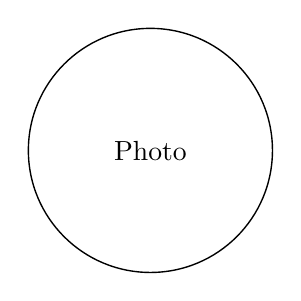
\begin{tikzpicture}
        \draw[line width=0.5pt] (0,0) circle (15.5mm);
        \node[text width=20mm, align=center] at (0,0) {Photo};
    \end{tikzpicture}%
}

%-------------------------------------------
%%%%%%  CV STARTS HERE  %%%%%%%%%%%%%%%%%%%%%%%%%%%%


\begin{document}

% Place the photo frame in absolute position
% Adjust the numbers (170, 250) to move the photo right/left and up/down
\begin{textblock}{25}(170, 2.6)
    \roundphoto
\end{textblock}

%----------HEADING-----------------
\begin{tabular*}{\textwidth}{L@{\extracolsep{\fill}}C@{\extracolsep{\fill}}R}
    \href{mailto:luca-andre.woiton@airbus.com}{luca-andre.woiton@airbus.com} &
    \multirow{3}{*}{\Huge \textbf{Luca Woiton}} &  \\
    +49 (0) 1575 5511893 & & \\
    \href{https://www.linkedin.com/in/lwoiton/}{Linkedin: in/lwoiton} & &
\end{tabular*}

%-----------EXPERIENCE-----------------
\section{Work Experience}
\resumeSubHeadingListStart
\resumeSubheading
{Mass Properties Engineer - Airbus Operations GmbH}{Bremen, Germany}
{Full-time}{Oct 2021 -- May 2023}
\resumeItemListStart
\resumeItemNH{Developed Python and Google Apps Script tools for weight calculations and database management}
\resumeItemNH{Created comprehensive mass model for A321XLR flight test campaign, earning AIRward recognition}
\resumeItemNH{Improved database granularity through semi-automated equipment installation tracking}
\resumeItemNH{Provided technical consultation on weight impacts across departments}
\resumeItemNH{Managed and analyzed complex aircraft modification data in cross-functional team settings}
\resumeItemListEnd

\resumeSubheading
{Dual Study Program - Airbus Operations GmbH}{Bremen, Germany}
{Engineering \& Apprenticeship}{Sep 2017 -- Oct 2021}
\resumeItemListStart
\resumeItemNH{Rotated through key aerospace functions: Procurement, Manufacturing, Materials \& Processes}
\resumeItemNH{Developed MATLAB/Simulink models for mechanical systems and automation processes}
\resumeItemNH{Combined engineering studies with IHK-certified aircraft mechanic training}
\resumeItemListEnd

%-----------EDUCATION-----------------
\section{Education}
\resumeSubHeadingListStart
\resumeSubheading
{42 - 42Prague - A very modern and disruptive IT school}{Prague, Czechia}
{Computer Software Engineering}{Jan 2023 -- Apr 2025}
\resumeItemListStart
\resumeItem{Technical Focus}{Systems Programming (C/C++), Data Structures \& Algorithms, Network Programming, Peer-to-peer and project based Learning}
\resumeItem{Projects}{}
\begin{itemize}[leftmargin=*]
\projectSubItem{Unix Shell - Built POSIX shell in C implementing command execution and pipe handling}
\projectSubItem{HTTP/1.1 server - Developed concurrent server in C++ with robust error handling}
\projectSubItem{3D Raycasting Engine - Created optimized graphics engine with texture mapping}
\end{itemize}
\resumeItemListEnd

\resumeSubheading
{HSB Hochschule Bremen}{Bremen, Germany}
{B.E. in Mechanical and Production Engineering}{Sep 2017 -- Oct 2021}
\resumeItemListStart
\resumeItem{Thesis}{MBSE framework development for wing mass estimation using modern software architecture}
\resumeItem{Technical Focus}{Engineering fundamentals, CAD/CAM, MATLAB/Simulink, measurement techniques}
\resumeItem{Projects}{}
\begin{itemize}[leftmargin=*]
\projectSubItem{Industrial surface treatment study for aircraft components}
\projectSubItem{Arduino-based control systems development}
\projectSubItem{Matlab windpark economical simulation program}
\projectSubItem{Mechatronical System simulation with MATLAB/Simulink}
\end{itemize}
\resumeItemListEnd

%-----------INVOLVEMENT-----------------
\section{Professional Involvement \& Projects}
\resumeSubHeadingListStartBullets
\resumeSubItem{Technical Advisory Board}
{Led apprentice association projects and organized professional team building events}
\resumeSubItem{Engineering Student Council}
{Mentored first-year students and supported academic initiatives}
\resumeSubItem{Language Learning Automation}
{Created system integrating PDF parsing, REST APIs, and OpenAI for automated learning materials}
\resumeSubHeadingListEnd

%--------SKILLS------------
\section{Skills}
\resumeSubHeadingListStart
\resumeSubItem{Programming}{C, C++, Python, JavaScript, Google Apps Script, MATLAB/Simulink}
\resumeSubItem{Technologies}{Git, Unix/Linux, SQL, VirtualBox, REST APIs}
\resumeSubItem{Engineering}{CAD/CAM, Mass Properties, Aircraft Systems, Airbus Product Structure, Manufacturing Processes}
\resumeSubItem{Soft Skills}{Cross-functional projects, Project management, Intercultural collaboration and teamwork, Intrinsically motivatied and diciplined, Peer-to-peer mentoring and learning}
\resumeSubItem{Languages}{German - native; English - C2; French - B1; Czech - A1.5}
\resumeSubHeadingListEnd

%-----------AWARDS-----------------
\section{Honors}
\resumeSubHeadingListStartBullets
\resumeSubItem{AIRward Recognition}
{Outstanding technical contributions to A321XLR flight test campaign at Airbus}
\resumeSubHeadingListEnd
%-------------------------------------------
\end{document}